\documentclass[a4paper,12pt,final]{article}
\usepackage{hyperref}
\usepackage{graphicx}
\usepackage{algorithmic}
\usepackage{verbatim}
\usepackage[small,compact]{titlesec}
\usepackage[small,it]{caption}
\newcommand{\assign}{\mathrel{\mathop:}=}

\setlength{\topmargin}{0in}
\setlength{\headheight}{0in}
\setlength{\headsep}{0in}
\setlength{\textheight}{7.7in}
\setlength{\textwidth}{6.5in}
\setlength{\oddsidemargin}{0in}
\setlength{\evensidemargin}{0in}
\setlength{\parindent}{0in}
%\setlength{\parskip}{0.0in}

\begin{document}

\title{Monty Carlo Simulation for Generating $\gamma$}
\date{}
\author{Matthew Wampler-Doty }

\maketitle
\setlength{\parskip}{0.15in}

This is a Monty Carlo simulation for calculating $\gamma$ for
use with \emph{Mathematica}.  We employ the following algorithm, where
$r$ and $X$ are given:\\

\begin{algorithmic}
\STATE $hits \gets$ 0
\STATE $total \gets$ 0
\WHILE {$total < X$}
             \STATE $(x,y) \gets $ random value
             $\in [-(r+0.5),r+0.5]^2$
             \STATE $\theta \gets$ random value $\in [0,2 \pi]$
             \STATE $e_1 \gets (x,y) + \frac{r}{2}\cdot (\cos\theta, \sin\theta)$
             \STATE $e_2 \gets (x,y) - \frac{r}{2}\cdot(\cos\theta,
             \sin\theta)$
             \IF {$e_1$ or $e_2$ are out of bounds} \STATE $continue$ \ENDIF
             \IF {$e_1$ or $e_2$ is in the subarray}
                    \STATE $hits \gets hits + 1$
             \ELSE
                    \STATE $m \gets  \tan \theta$
                    \STATE $k \gets y - m x$
                    \STATE $l \gets \lambda x. m x + k$
                    \STATE $l^{-1}\gets \lambda y. \frac{y - k}{m}$
                    \STATE $a \gets \left(-0.5,l(-0.5)\right)$
                    \STATE $b \gets \left(0.5,l(0.5)\right)$
                    \STATE $c \gets \left(l^{-1}(0.5),0.5\right)$
                    \STATE $d \gets \left(l^{-1}(-0.5),-0.5\right)$
                    \IF {$a$ or $b$ or $c$ or $d$ are on
                      $\overline{e_1 e_2}$ and in the subarray}
                       \STATE $hits \gets hits + 1$
                    \ENDIF
             \ENDIF
             \STATE $total \gets total + 1$
\ENDWHILE
\RETURN $hits/X$
\end{algorithmic}
The following is what is meant by the variables in this algorithm:
\begin{itemize}
\item $r$ is the length of the cosmic ray
\item $(x,y)$ is the center of the cosmic ray
\item $\theta$ is the direction of the cosmic ray
\item $e_1$ and $e_2$ are the ends of the cosmic ray
\item $m$ and $k$ are the slope and intercept of the line
  $\overline{e_1e_2}$
\item $l$ is the line through $\overline{e_1e_2}$, and $l^{-1}$ is its inverse
\item $a$,$b$,$c$, and $d$ are as indicated in Figure \ref{drawing2};
  if one of these points is in the subarray, then we know that there
  was a collision with the cosmic ray
\end{itemize}
What follows is an implementation of the main loop of the algorithm in
python:
\pagebreak
\begin{figure}[hb]
\centering
    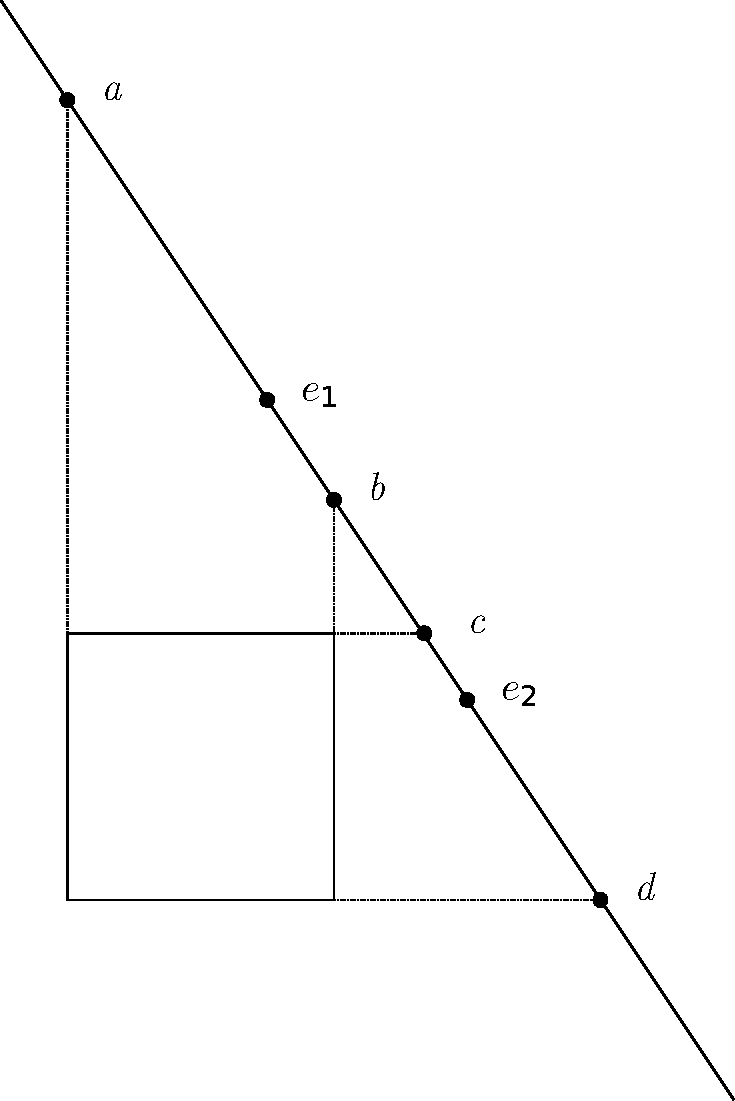
\includegraphics[height=1\textheight]{drawing2.pdf}
\caption{Points to check to see if the cosmic ray collides with subarray}\label{drawing2}
\end{figure}
\clearpage
\begin{verbatim}
from random import seed, uniform
from math import pi, cos, sin, tan
from numpy import array,arange
from numpy.linalg import norm

seed()

def gammamc(r,X):
    hits = 0.0
    total = 0
    while total < X:
          x = uniform(-(r+0.5),r+0.5)
          y = uniform(-(r+0.5),r+0.5)
          theta = uniform(0,2*pi)
          e1 = array([x,y]) + r/2 * array([cos(theta),sin(theta)])
          e2 = array([x,y]) - r/2 * array([cos(theta),sin(theta)])
          if isOutOfBounds(r,e1) | isOutOfBounds(r,e2): continue
          if isInSubarray(e1) | isInSubarray(e2): hits+=1
          else:
             m = tan(theta)
             k = y - m*x
             l = (lambda x: m*x + k)
             invl = (lambda y: (y - k)/m)
             a = [-0.5,l(-0.5)]
             b = [0.5,l(0.5)]
             c = [invl(0.5),0.5]
             d = [invl(-0.5),-0.5]
             isOnLine = (lambda pt: (min(e1[0],e2[0]) <= pt[0]) 
                                and (pt[0] <= max(e1[0],e2[0])) 
                                and (min(e1[1],e2[1]) <= pt[1])
                                and (pt[1] <= max(e1[1],e2[1])) )
             if (    (isOnLine(a) and isInSubarray(a))
                  or (isOnLine(b) and isInSubarray(b))
                  or (isOnLine(c) and isInSubarray(c))
                  or (isOnLine(d) and isInSubarray(d))): hits += 1
          total+=1
    return hits/X

\end{verbatim}

 \pagebreak
Some functions that we call here have yet to be defined.  We will
go over their motivation before providing them.

\textbf{Out of Bounds}: When picking the ends of the cosmic ray ($e_1$
and $e_2$), they might not be in bounds.  To be in bounds it must be
possible to reach the subarray, and this area is located in Figure
\ref{drawing1}.
We have normalized the subarray to a $1\times 1$ square centered at
$0$, so here $s = 1$ and $x = r$.  A point $(x,y)$ is out of bounds if and
only if one of the following hold:
\begin{center}
\begin{tabular}{ccc}
  $x \leq -(r + 0.5)$ &  & $r + 0.5 \leq x$ \\
  $y \leq -(r+0.5)$ & & $r + 0.5 \leq y$ \\
\multicolumn{3}{c}{$||(x,y)-\vec{cr}|| \leq r \leq ||(x,y)-\vec{sa}|| $}
\end{tabular}
\end{center}
Where $\vec{cr}$ is a corner of $[-(r+0.5),r+0.5]^2$ and $\vec{sa}$ is
a corner of $[-0.5,0.5]^2$.

\begin{figure}[hb]
\centering
    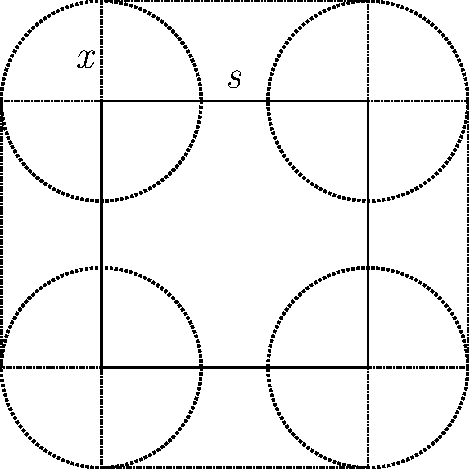
\includegraphics[width=0.6\textwidth]{drawing.pdf}
\caption{Area where it is possible for a cosmic ray to hit a subarray}\label{drawing1}
\end{figure}
\pagebreak
This is the python code that implements this:

\begin{verbatim}
def isOutOfBounds(r,pt):
    x,y=pt
    if (    (x <= -(r + 0.5)) or (r + 0.5 <= x)
         or (y <= -(r + 0.5)) or (r + 0.5 <= y) ): return True
    for cr,sa in [[array([xo*(r+0.5),yo*(r+0.5)]),
                   array([xo*0.5,yo*0.5])] for xo in [-1,1] 
                                           for yo in [-1,1]]:
        if ((norm(pt-cr) <= r) and (r <= norm(pt-sa))): return True
    return False

\end{verbatim}

 
Finally, to check if a point $(x,y)$ is in the subarray, we just need
to verify that:
\begin{eqnarray*}
-0.5 \leq x \leq 0.5 & \textup{ and } & -0.5 \leq y \leq 0.5
\end{eqnarray*}

\begin{verbatim}
def isInSubarray(pt):
    x,y=pt
    return (     (-0.5 <= x) and (x <= 0.5) 
             and (-0.5 <= y) and (y <= 0.5) )

\end{verbatim}

 
We may now run the simulation and record the contents in a tab
separated value file.

This code can take a long time to run, so we will set up a tab
separated value file (TSV) and output to there.  We then use
\emph{Mathematica} to do further data analysis.

\begin{verbatim}
import os
fp = open("gammamc.tsv","w")
for x in arange(0,100,0.01): 
     fp.write("%g\t%f\n" % (x,gammamc(x,1000)))
     fp.flush()
     os.fsync(fp)
 fp.close()
\end{verbatim}

 
\end{document}